\documentclass{article}
\usepackage[T1]{fontenc}
\usepackage{amssymb}
\usepackage{hyperref}
\usepackage{amsmath}
\usepackage[utf8]{inputenc}
\usepackage[polish]{babel}
\usepackage{graphicx}
\usepackage{float}
%{Informatyka stosowana 2020, I st., semestr VI}


\author{
	{Dominik Gałkowski, 247659} \\
	{Jan Śladowski, 247806}\\ 
{Prowadzący: dr inż. Marcin Kacprowicz}
}

\title{Komputerowe systemy rozpoznawania 2024/2025\\Projekt 1. Klasyfikacja dokumentów tekstowych}
\begin{document}
\maketitle


\section{Cel projektu}
\indent Celem projektu jest przygotowanie aplikacji, która będzie dokonywała klasyfikacji zbioru dokumentów tekstowych metodą k-NN. Jej zadaniem będzie przydzielenie obiektu do odpowiedniej klasy. W trakcie działania programu konieczne będzie dokonanie ekstrakcji wektorów cech ze zboiru artykułów Reuters \cite{reuters}. \\

\section{Klasyfikacja nadzorowana metodą $k$-NN.  Ekstrakcja cech, wektory cech}
Metoda k-NN (k-Nearest Neighbors) jest algorytmem leniwym, co oznacza, że nie tworzy wewnętrznej reprezentacji danych uczących, tylko przechowuje wszystkie wzorce uczące. Dopiero po pojawieniu się wzorca testowego, dla którego wyznaczana jest odległość względem wszystkich wzorców uczących, algorytm poszukuje rozwiązania. \cite{knn}. Algorytm k-NN wymaga dwóch kluczowych parametrów, metryki, za pomocą, której wyznacza odległości obiektu testującego od wszystkich wzorców uczących oraz liczby sąsiadów k, czyli elementów do których badany element ma najbliżej. Decyzja klasyfikacyjna opiera się na najczęstszej klasie wśród k najbliższych sąsiadów. W przypadku naszego projektu odległość pomiędzy obiektami oznacza skalę podobieństwa tekstów.

W projekcie ekstrakcja cech charakterystycznych tekstu jest dokonywana poprzez stworzenie wektora cech, opisanego na podstawie następujących cech:
\begin{enumerate}
    \item Długość tekstu - cecha ta oznacza liczbę słów, z których składa się dany artykuł, co pozwala na porównanie długości różnych tekstów.
        \begin{equation}
            len = \sum_{i=0}^{n} x_i
        \end{equation}
        gdzie \( x \) = liczba liter \( \geq 3 \), \( n \) = liczba słów w tekście.
    \item Dominująca waluta - cecha ta reprezentowana jest poprzez nazwę waluty, ze zbioru walut kluczowych, która pojawia się najczęściej w badanym artykule. Na przykład w przypadku, gdy w badanym tekście pojawi się dwukrotnie słowo "U.S. Dollar" i tylko raz "Japanese Yen" to dla tej cechy zostanie zwrócona wartość tekstowa "U.S. Dollar".
        \begin{equation}
            w = \arg\max_{w \in W} f(w)
        \end{equation}
        gdzie W - zbiór walut kluczowych, \( f(w) \)  - liczba wystąpień waluty \( w \) w tekście.
    \item Nazwy miejsca - cecha ta jest reprezentacją tekstową wszystkich miejsc, np. nazw miast lub regionów pojawiających się ze zbioru miejsc kluczowych. Przykład: "AMR Corp will hold a press conference this morning in New York at 0900 EST, a company spokesman said." wynikiem dla tego cytatu będzie zbiór \( M' = \{ \text{New York} \} \). 
        \begin{equation}
            M' =  x \in M  \land x \in T
        \end{equation}
        gdzie M - zbiór miejsc kluczowych, T - zbiór słów znajdujących się w tekście, \( x \) = liczba liter \( \geq 3 \).
    \item Liczba unikalnych słów - cecha oznaczająca wystąpienia słów unikalnych, czyli takich, które nie pojawiąją się więcej niż jeden raz w tekście. Przykład: "AMR Corp will hold a press conference this morning in New York at 0900 EST, a company spokesman said. And the next week also in New York", słowa "New York" nie zostaną zliczone.
        \begin{equation}
            uk = \mid x : x \in T \land f(x) = 1 \mid
        \end{equation}
        gdzie T - zbiór słów znajdujących się w tekście, \( f(x)\)  - funkcja zwracająca liczbę wystąpień słowa x w tekście, \( x \) = liczba liter \( \geq 3 \).
    \item Średnia długość słowa - cecha opisująca średnią długość słów w badanym tekście.
     \begin{equation}
            al = \frac{\sum_{i=0}^{m} a_i}{\sum_{i=0}^{n} x_i}
        \end{equation}
        gdzie \( a_i \) - litera, \( x \) - liczba liter \( \geq 3 \), \( n \) = liczba słów w tekście, \( m \) = liczba liter w tekście.
    \item Liczba słów kluczowych w pierwszych 3 zdaniach - cecha ta oznacza bezwględną liczbę wystąpień słów ze zbioru słów kluczowych w pewnym fragmencie tekstu (pierwsze 3 zdania).
        \begin{equation}
            fw = \ \mid x : x \in K \wedge x \in T_{\text{y}} \mid
        \end{equation}
        gdzie K - zbiór słów kluczowych, \( T_y \) - zbiór słów znajdujący się w pierwszych trzech zdaniach tekstu, \( x\) = liczba liter \( \geq 3 \).
    \item Liczba słów zaczynających się wielką literą - cecha ta oznaczą liczbę wystąpień słów zaczynających się wielką literą, nie uzwlędniając przy tym słów rozpoczynających nowe zdanie.
        \begin{equation}
            bw = \sum_{i=0}^{n} x_i
        \end{equation}
        gdzie \( x \) = słowo zaczynające się wielką literą, \( n \) = liczba słów zaczynających się wielka literą w tekście
    \item Pierwsze kluczowe słowo w tekście - cecha opisująca pierwsze znalezione słowo znajdujące się w zbiorze słów kluczowych. Przykład: "AMR Corp will hold a press conference this morning in New York at 0900 EST, a company spokesman said." wynikiem dla tego cytatu będzie \(x_{first} \) = New York.
       \begin{equation}
            x_{first} = \min \{x: x \in K \land x \in T \}
        \end{equation}
        gdzie K - zbiór słów kluczowych, T - zbiór słów znajdujących się w tekście, \( x \) = liczba liter \( \geq 3 \).
    \item Liczba słów kluczowych - cecha ta oznacza bezwzględną liczbę wystąpień słów ze zbioru słów kluczowych. 
        \begin{equation}
            kw = \ \mid x : x \in K \land x \in T \mid
        \end{equation}
        gdzie K - zbiór słów kluczowych, T - zbiór słów znajdujących się w tekście, \( x \) = liczba liter \( \geq 3 \).
    \item Względna liczba słów kluczowych - cecha która reprezentuje stosunek słów kluczowych do długości całego tekstu. 
        \begin{equation}
            rw = \frac{ \mid x : x \in K \land x \in T \mid}{ \sum_{i=0}^{n} x_i}
        \end{equation}
       gdzie K - zbiór słów kluczowych, \( x \) = liczba liter \( \geq 3 \), T - zbiór słów znajdujących się w tekście, \( n \) = liczba słów w tekście
    \item Nazwiska - cecha ta jest reprezentacją tekstową wszystkich nazwisk pojawiających się ze zbioru nazwisk kluczowych. Przykład: "Wallis was quoted as saying the Reagan Administration wants Japanese cooperation so the White House can ensure any U.S." wynikiem dla tego cytatu będzie zbiór \( N' = \{ \text{Reagan} \} \).
    \begin{equation}
            N' =  x \in N \land x \in T
        \end{equation}
        gdzie N - zbiór nazwisk kluczowych, T - zbiór słów znajdujących się w tekście, \( x \) = liczba liter \( \geq 3 \).
\end{enumerate}

Wektor cech będzie miał postać: 
        \begin{equation}
          v = [c1, c2, c3, c4, c5, c6, c7, c8, c9, c10, c11]
        \end{equation}


\section{Miary jakości klasyfikacji}
W celu określenia jakości przeprowadzonej klasyfikacji należy skorzystać z czterech miar jakości. W trakcie omawiania tej sekcji będziemy się posługiwać symbolami, które będą oznaczać klasy, do których można przypisać dany tekst (J - Japonia, F - Francja, W - Niemcy Zachodnie, C - Kanada, U - USA, UK - Wielka Brytania). 

\subsection{Dokładność (Accuracy)}
Dokładność to miara, która określa jaka część obiektów, ze wszystkich zaklasyfikowanych, została zaklasyfikowana poprawnie. Dokładność jest obliczana dla wszystkich klas jednocześnie i przyjmuje wartości z zakresu \([0, 1]\). Wyższa wartość dokładności oznacza, że ogólny procent poprawnie sklasyfikowanych obiektów jest większy, co sugeruje, że skuteczność klasyfikatora jest większa.
\begin{equation}
    ACC = \frac {TP}{TP + N}
\end{equation}
gdzie \(ACC\) - accuracy, \(TP\) - liczba wszystkich poprawnie sklasyfikowanych tekstów, \(N\) - liczba niepoprawnie sklasyfikowanych tekstów. \\
\subsection{Precyzja (Precision)}
Dzięki precyzji dowiadujemy się, ile wśród obiektów sklasyfikowanych do danej klasy jest rzeczywiście tej klasy. Precyzja jest obliczana dla wszystkich klas oddzielnie i przyjmuje wartości z zakresu \([0\% -100\%]\). Im wyższy współczynnik precyzji, tym mniej błędnych klasyfikacji do danej klasy.
\begin{equation}
    PPV_x = \frac {TP_x}{TP_x + N_x}
\end{equation}
gdzie \(PPV_x\) - precision dla danej klasy \(x\), \(TP_x\) - liczba poprawnie sklasyfikowanych tekstów klasy \(x\), \(N_x\) - liczba niepoprawnie sklasyfikowanych  tekstów do klasy \(x\), \(x \in \{ \text{C, J, U, F, W, UK} \}\).
\subsection{Czułość (Recall)}
Czułość opisuje jaki jest udział poprawnie sklasyfikowanych obiektów wśród wszystkich obiektów tej klasy. Czułość jest obliczana dla wszystkich klas oddzielnie i przyjmuje wartości z zakresu \([0, 1]\). Wyższa wartość czułości oznacza, że klasyfikator skuteczniej wykrywa wszystkie przypadki danej klasy, co oznacza zmniejszenie liczby pominiętych istotnych obiektów.
\begin{equation}
    TPR_x = \frac {TP_x}{TP_x + NF_x}
\end{equation}
gdzie \(TPR_x\) - recall dla danej klasy \(x\), \(TP_x\) - liczba poprawnie sklasyfikowanych tekstów klasy \(x\), \(NF_x\) - liczba tekstów klasy \(x\), które zostały przypisane do innej klasy, \(x \in \{ \text{C, J, U, F, W, UK} \}\). 
\subsection{F1}
F1 to średnia harmoniczna pomiędzy precyzją a czułością, pozwalająca ocenić równowagę między nimi.  F1 jest obliczana dla wszystkich klas oddzielnie i przyjmuje wartości z zakresu \([0, 1]\). Im wyższa wartość miary F1, tym lepsza równowaga pomiędzy precyzją, a czułością
\begin{equation}
    F1_x = \frac{2 \times PPV_x \times TPR_x}{PPV_x + TPR_x}
\end{equation}
gdzie \(F1_x\) - miara F1 dla danej klasy \(x\), \(x \in \{ \text{C, J, U, F, W, UK} \}\). 

\subsection{Przykład z wykorzystaniem miar jakości klasyfikacji}
Mamy trzy zbiory, na ich podstawie obliczymy accuracy oraz precision, recall i F1 dla tekstów przypisanych do klasy Japonii: 
\begin{enumerate}
    \item Zbiór tekstów przypisanych jako Japonia \( \{ \text{J, J, J, F, U} \} \).
    \item Zbiór tekstów przypisanych jako Francja \( \{ \text{F, F, F, J} \} \).
    \item Zbiór tekstów przypisanych jako USA \( \{ \text{U, U, F, F} \} \).
\end{enumerate}

\begin{table}[h!]
    \centering
    \begin{tabular}{|c|c|c|c|}
        \hline
        - & \textbf{\(TP_X\)} & \textbf{\(N_X\)} & \textbf{\(NF_X\)} \\
        \hline
        \textbf{Japonia (J)}  & \( TP_J = 3 \) & \( N_J = 2 \) & \( NF_J = 1 \) \\
        \hline
        \textbf{Francja (F)}  & \( TP_F = 3 \) & \( N_F = 1 \) & \( NF_F = 3 \) \\
        \hline
        \textbf{USA (U)}      & \( TP_U = 2 \) & \( N_U = 2 \) & \( NF_U = 1 \) \\
        \hline
    \end{tabular}
    \caption{Wartości dla klasyfikacji tekstów}
\end{table}



gdzie \(TP_x\) - liczba poprawnie sklasyfikowanych tekstów klasy \(x\), \(N_x\) - liczba niepoprawnie sklasyfikowanych  tekstów do klasy \(x\), \(NF_x\) - liczba tekstów klasy \(x\), które zostały przypisane do innej klasy, \(x \in \{ \text{C, J, U, F, W, UK} \}\).

\begin{flushleft}
- \(TP = 3 + 3 + 2 = 8\) (suma wszystkich poprawnie sklasyfikowanych tekstów),\\
- \(N = 2 + 1 + 2 = 5\) (suma wszystkich tekstów przypisanych do niewłaściwej klasy).

\[
    ACC = \frac{TP}{TP + N} = \frac{8}{13} \approx 62\%
\]

- \(TP_J = 3\) (Liczba tekstów poprawnie sklasyfikowanych do Japonii),\\
- \(N_J = 2\) (Liczba tekstów niepoprawnie przypisanych do Japonii).

\[
    PPV_J = \frac{TP_J}{TP_J + N_J} =\frac{3}{5} = 0.6
\]

- \(TP_J = 3\) (Liczba tekstów poprawnie przypisanych do Japonii),\\
- \(NF_J = 1\) (Liczba tekstów klasy Japonia, które zostały błędnie przypisane do innej klasy).

\[
    TPR_J = \frac{TP_J}{TP_J + NF_J} = \frac{3}{4} = 0.75
\]
\[
    F1_J = \frac{2 \times PPV_J \times TPR_J}{PPV_J + TPR_J} = \frac{0.9}{1.35} \approx 0.67
\]

\end{flushleft}

\section{Metryki i miary podobieństwa tekstów w klasyfikacji}
Metoda klasyfikacji k-NN polega na znajdowaniu k najbliższych sąsiadów, kluczową rolę w tym procesie odgrywają metryki oraz miary, które są wykorzystywane do ustalenia stopnia zgodności pomiędzy obiektami. Metryki umożliwiają obliczenie odległości między wektorami liczbowymi. Natomiast w przypadku cech tekstowych, zanim będzie można obliczyć ich podobieństwo, należy dokonać ich transformacji na wartości liczbowe. Umożliwiają to miary, które określają podobieństwo między ciągami znaków.

\subsection{Metryki}
\begin{enumerate}
    \item Metryka euklidesowa - w celu obliczenia odległości \(\rho_E(v1, v2)\) między dwoma wektorami \(v1, v2\) należy obliczyć pierwiastek kwadratowy z sumy kwadratów różnic ich składowych zgodnie ze wzorem:
        \begin{equation}
      \rho_E(v1, v2) = \sqrt{\sum_{i=1}^{n} (v1_i \underset{m}{-} v2_i)^2}  
        \end{equation}
        gdzie \(n\) - liczba cech w wektorach.
        
    \item Metryka uliczna - w celu obliczenia odległości \(\rho_M(v1, v2)\) między dwoma wektorami \(v1, v2\) należy obliczyć sumę wartości bezwzględnych różnic cech zgodnie ze wzorem:
        \begin{equation}
          \rho_M(v1, v2) = \sum_{i=1}^{n} |v1_i \underset{m}{-} v2_i|
        \end{equation}
        gdzie \(n\) - liczba cech w wektorach.
        
    \item Metryka Czebyszewa - w celu obliczenia odległości \(\rho_C(v1, v2)\) między dwoma wektorami \(v1, v2\) należy obliczyć maksymalną wartość bezwzględnych różnic cech zgodnie ze wzorem:
        \begin{equation}
          \rho_C(v1, v2) = \max_{i = 1,...,n} |v1_i \underset{m}{-} v2_i|
        \end{equation}
        gdzie \(n\) - liczba cech w wektorach.
\end{enumerate}
gdzie 
\[
    v1_i \underset{m}{-} v2_i = 
    \begin{cases}
    v1_i - v2_i & \text{dla } v1_i, v2_i \in \mathbb{R} \\
    1 - sim_w(v1_i, v2_i) & \text{jeśli } v1_i, v2_i \text{ są tekstami}\\
    1 - sim_z(v1_i, v2_i) & \text{jeśli } v1_i, v2_i \text{ są zbiorami tekstów}
    \end{cases}
\]
gdzie \(v1_i\), \(v2_i\) - i-ta składowa wektorów cech \(v1\) oraz \(v2\),\\ \(sim_w\) - podobieństwo tekstów obliczone uogólnioną miarę n-gramów z ograniczeniami (pkt 4.2),\\ \(sim_z\) - podobieństwo zbiorów wyrazów obliczone miarą podobieństwa zdań (pkt 4.3). \\
W celu poprawnego przeprowadzenia obliczeń dla metryk należy uprzednio przeprowadzić normalizację cech wektórów, tak aby żadna z cech nie była dominująca. Wektory zostaną znormalizowane za pomocą metody min-max scaling do zakresu [0, 1].\\
Załóżmy, że mamy dwa wektory cech:
\begin{enumerate}
    \item \(v1 = (1, 2, 30)\)
    \item \(v2 = (4, 6, 3)\)
\end{enumerate}
\[
    c_{\min} = 1, \quad c_{\max} = 30
\]
gdzie c to cecha składowa wektora \(v1\) lub \(v2\). \\
Aby otrzymać znormalizowane wartości należy skorzystać z wzoru:
\begin{equation}
    c' = \frac{c - c_{min}}{c_{max} - c_{min}}
\end{equation}
Znormalizowana postać wektorów:
\begin{enumerate}
    \item \(v1' = (0.000, 0.034, 1.000)\)
    \item \(v2' = (0.103, 0.172, 0.069)\)
\end{enumerate} 
Z wykorzystaniem powyższych wektorów otrzymujemy:
\[
     \rho_E(v1, v2) = \sqrt{(0.000 - 0.103)^2 + (0.034 - 0.172)^2 + (1.000 - 0.069)^2} = 
\]
\[
       = \sqrt{0.946} \approx 0.947
\]
\[
    \rho_M(v1, v2) = |0.000 - 0.103| + |0.034 - 0.172| + |1.000 - 0.069| = 1.172
\]
\[
    \rho_C(v1, v2) = \max(|0.000 - 0.103|, |0.034 - 0.172|, |1.000 - 0.069|) = 
\]
\[
     = \max(0.103, 0.138, 0.931) = 0.931
\]
\\
Metryka euklidesowa, uliczna oraz Czebyszewa przyjmują wartości z zakresu \([0, \infty)\). Im otrzymana wartość jest mniejsza, tym oba wektory cech są do siebie bardziej podobne.

\subsection{Uogólniona miara n-gramów z ograniczeniami}
Wykorzystując uogólnioną miarę n-gramów z ograniczeniami możemy pewną liczbą wyrazić podobieństwo dwóch łańcuchów znaków. Ta miara przyjmuje wartości z zakresu \([0,1]\), przy czym wartości wyższe oznaczają większe podobieństwo pomiędzy badanymi łańcuchami znaków. Krańcowe wartości oznaczają: 0 – różne łańcuchy znaków, 1 - identyczne łańcuchy znaków. Przekształcenie cech tekstowych na wartości numeryczne umożliwia obliczenie ich wpływu na odległości między wektorami. Odległość pomiędzy dwoma łańcuchami znaków możemy określić poprzez:
\begin{equation}
    d = 1 - sim_w(s1, s2)
\end{equation}
gdzie \(sim_w(s1,s2)\) oznacza uogólnioną miarę n-gramów z ograniczeniami
\begin{equation}
    \mu_N(s1, s2) = f(N, n_1, n_2) \sum_{i=n_1}^{n_2} \sum_{j=1}^{N(s1) - i + 1} h(i, j)
\end{equation}
gdzie \( s1, s2\) - cechy, które przyjmują wartości tekstowe;
\begin{equation} 
f(N, n_1, n_2) = \frac{2}{(N - n_1 + 1)(N - n_1 + 2) - (N - n_2 + 1)(N - n_2)}
\end{equation}
wyraża odwrotność liczby możliwych podciagów o długosciach od \(n_1\) do \(n_2\)
\(1 \leq n_1 \leq n_2 \leq N\); \\
\(h(i,j) = 1\) jeśli \(i\)-elementowy podciag w słowie s1 zaczynajacy sie od \(j\)-tej
pozycji w słowie \(s_1\) pojawia sie przynajmniej raz w słowie \(s_2\) (inaczej
\(h(i,j) = 0\));\\
\(N(s1), N(s2)\) - oznaczają liczbę liter w słowach \( s1\) i \(s2\);\\
\(N = \max \{N(s1), N(s2)\}\).\\


Załóżmy, że mamy dwa wektory cech (wektory powinny być znormalizowane, ale na potrzeby tego przykładu zostało to pominięte):
\begin{enumerate}
    \item \(v1 = (1, KARTON, 3)\)
    \item \(v2 = (4, KARNISZ, 3)\)
\end{enumerate}
Traktując drugą cechę jako łańcuchy znaków, mamy:
\[
s_1 = \{K, A, R, T, O, N\}, \quad s_2 = \{K, A, R, N, I, S, Z\}
\]
czyli:\\
\[
N(s_1) = 6, N(s_2) = 7, N = \max \{N(s_1), N(s_2)\} = 7
\]
Obliczając podobieństwo przyjmujemy \(n_1 = 2\) oraz \(n_2 = 3\) 
\[
    \mu_N(s_1, s_2) = \frac{2}{(7 - 2 + 1)(7 - 2 + 2) - (7 - 3 + 1)(7 - 3)} \sum_{i=2}^{3} \sum_{j=1}^{6 - i + 1} h(i, j) = 
 \]
 \[
     = \frac{2 + 1}{11} \approx 0.27.
 \]
 ponieważ w \(s_2\) występują poniższe podciągi z \(s_1\)\\
 2 - 2-elementowe KA, AR;\\
 1 - 3-elementowy KAR;\\
 \\Wówczas odległość euklidesowa pomiędzy wektorami wynosi:
 \[
     \rho_E(v1, v2) = \sqrt{(1-4)^2 + (1 - 0.27)^2 + (3-3)^2} = \sqrt{9 + 0.73 + 0} = 
\] 
\[
     = \sqrt{9.73} \approx 3.12
\] 

\subsection{Miara podobieństwa zdań}
Wykorzystując uogólnioną miarę podobieństwa zdań, traktowanych jako zbiory (a nie ciągi) wyrazów, możemy pewną liczbą wyrazić stopień podobieństwa pomiędzy dwoma zbiorami słów. Miara ta przyjmuje wartości z zakresu \([0,1]\), gdzie wyższe wartości oznaczają większe podobieństwo między porównywanymi zbiorami. Krańcowe wartości interpretujemy następująco: 0 – zbiory zupełnie różne, 1 – zbiory identyczne pod względem zestawu użytych słów. Przekształcenie cech tekstowych na wartości numeryczne umożliwia analizę ich wpływu na odległości w przestrzeni wektorowej. Odległość pomiędzy dwoma zbiorami wyrazów możemy określić za pomocą następującej formuły:
\begin{equation}
    d = 1 - sim_z(z1, z2)
\end{equation}
gdzie \(sim_z(z1,z2)\) oznacza miarę podobieństwa zdań\\
\begin{equation} 
\mu_{NZ}(z_1, z_2) = \frac{1}{N} \sum_{i=1}^{N(z_1)} \max_{j = 1, \ldots, N(z_1)} \mu_N(s_{1i}, s_{2j})
\end{equation}
gdzie:\\
 $s_{1i}$ – $i$-ty wyraz w zbiorze $z_1$;\\
 $s_{2j}$ – $j$-ty wyraz w zbiorze $z_2$;\\
 $\mu_N(s_{1i}, s_{2j})$ – wartość funkcji (22) dla $(s_{1i}, s_{2j})$;\\
 $N(z_1), N(z_2)$ – liczba słów w zbiorach $z_1$, $z_2$;\\
 $N = \max\{N(z_1), N(z_2)\}$.\\
Załóżmy, że mamy dwa wektory cech (wektory powinny być znormalizowane, ale na potrzeby tego przykładu zostało to pominięte):
\begin{enumerate}
    \item \(v_1 = (1, \text{ kot je}, 3)\)
    \item \(v_2 = (4, \text{ kot pije wodę}, 3)\)
\end{enumerate}
Traktując drugą cechę jako zbiór wyrazów, mamy:
\[
z_1 = \{\text{kot}, \text{je}\}, \quad z_2 = \{\text{kot}, \text{pije}, \text{wodę}\}
\]
czyli:
\[
N(z_1) = 2, \quad N(z_2) = 3, \quad N = \max\{N(z_1), N(z_2)\} = 3
\]
Wartość podobieństwa zbiorów:
\[
\mu_{NZ}(z_1, z_2) = \frac{1}{3}\sum_{i=1}^{3} \max_{j = 1, 2} \mu_N(s_{1i}, s_{2j}) = \frac{1 + 0.2 + 0}{3} = 0.4
\]

gdzie
\[
\begin{aligned}
\max \{\mu_N(\text{kot}, \text{kot}), \mu_N(\text{je}, \text{kot})\} = 1.0 \\
\max \{\mu_N(\text{kot}, \text{pije}), \mu_N(\text{je}, \text{pije})\} = 0.2 \\
\max \{\mu_N(\text{kot}, \text{wodę}), \mu_N(\text{je}, \text{wodę})\} = 0 \\
\end{aligned}
\]
Wówczas odległość euklidesowa pomiędzy wektorami wynosi:
\[
\rho_E(v_1, v_2) = \sqrt{(1 - 4)^2 + (1 - 0.4)^2 + (3 - 3)^2} = \sqrt{9 + 0.36 + 0} = \sqrt{9.25} \approx 3.06
\]

\section{Wyniki klasyfikacji dla różnych parametrów wejściowych}
W tej sekcji przeprowadzono eksperymenty polegające na dokonaniu klasyfikacji tekstów dla zbioru składającego się z 13441 artykułów, przy czym są to artykuły, które posiadają etykietę tylko jednego kraju (USA, Wielka Brytania, Kanada, Francja, Niemcy Zachodnie, Japonia). Celem tego badania było przeprowadzenie analizy wpływu parametrów wejściowych algorytmu k-najbliższych sąsiadów na jakość klasyfikatora, którą można ocenić poprzez cztery miary (\(accuracy\), \(precision\), \(recall\), \(F1\)). \\
Badanie przeprowadzono w oparciu o różne warianty konfiguracji parametów wejściowych, zgodnie z punktami 3–8 zawartymi w opisie Projektu 1. Uwzględniono m.in. różne wartości parametru \(k\), różny podział zbioru pomiędzy uczący, a testowy, różne metryki oraz różne podzbiory cech. Eksperymenty polegają na tym, że w każdym z nich będzie zmieniany tylko jeden parametr, którego wpływ będzie aktualnie badany.
Oznaczenia użyte w tabelach to: ACC - opisane w (13),  \( \text{PPV}_x \) - (14), \( \text{TPR}_x \) - (15), \( \text{F1}_x \) - (16), U - teksty o Stanach Zjednoczonych, UK - teksty o Wielkiej Brytanii, C - teksty o Kanadzie, J - teksty o Japonii, F - teksty o Francji, W - teksty o Niemczech Zachodnich, a - średnia z wszystkich tekstów.
\\
Przykładowy wektor po ekstrakcji i normalizacji cech, który jest wykorzystywany w procesie klasyfikacji, wygląda następująco:
\[
    v = [ 0.04584717607973422, dlrs, [ florida, florida], 0.09576427255985268,
\]
\[
     0.5597984105446793, 0.047619047619047616, 0.036312849162011177, florida,
\]
\[
     0.058823529411764705, 0.15584415584415584, [] ]
\]
\subsection{Różne wartości parametru \(k\)}
W poniższej tabeli przedstawiono wpływ różnych wartości parametru \(k\) na dokładność klasyfikacji tekstów. Eksperymenty przeprowadzono przy stałych pozostałych ustawieniach: podziale zbioru danych na 60\% zbioru uczącego i 40\% zbioru testowego, metryce euklidesowej oraz zakresie długości n-gramów od \(n_1 = 2\) do \(n_2 = 4\). \\
\begin{table}[h!]
    \centering
    \begin{tabular}{|c|c|c|c|c|c|c|c|c|}
    \hline
    \textbf{Parametr k} & \textbf{\(1\)} & \textbf{\(2\)} & \textbf{\(3\)} & \textbf{\(5\)}  & \textbf{\(9\)}  & \textbf{\(15\)} & \textbf{\(25\)} \\ \hline
    ACC [\%] & 85,53 & 85,53 & 88,23 & 88,94 & 89,27 & 89,14 & 88,84\\ \hline
    PPV\(_U\) & 0,9999 & 0,9999 & 0,9101 & 0,9093 & 0,9061 & 0,9047 & 0,9025\\ \hline
    TPR\(_U\) & 0,9310 & 0,9310 & 0,9640 & 0,9733 & 0,9796& 0,9794 & 0,9806\\ \hline
    F1\(_U\) & 0,9203 & 0,9203 & 0,9363 & 0,9402 & 0,9414& 0,9406 & 0,9399\\ \hline
    PPV\(_C\) & 0,4794 & 0,4794 & 0,6500 &  0,7222 & 0,7585& 0,7536& 0,7938\\ \hline
    TPR\(_C\) & 0,4646 & 0,4646 & 0,4800 &  0,4800& 0,4831& 0,4800& 0,4738\\ \hline
    F1\(_C\) & 0,4719 & 0,4719 & 0,5522 &  0,5767& 0,5902& 0,5865& 0,5934\\ \hline
    PPV\(_{UK}\) & 0,6799 & 0,6799 & 0,7692 & 0,8036& 0,8465& 0,8543& 0,8408\\ \hline
    TPR\(_{UK}\) & 0,6160 & 0,6160 & 0,6077 &  0,6105& 0,5939& 0,5829& 0,5691\\ \hline
    F1\(_{UK}\) & 0,6464 & 0,6464 & 0,6790 &  0,6939& 0,6981& 0,6929& 0,6787\\ \hline
    PPV\(_F\) & 0,6087 & 0,6087 & 0,7403 & 0,7600& 0,8000& 0,7746& 0,7123\\ \hline
    TPR\(_F\) & 0,5545 & 0,5545 & 0,5644 & 0,5644& 0,5545& 0,5446& 0,5149\\ \hline
    F1\(_F\) & 0,5803 & 0,5803 & 0,6404 &  0,6477& 0,6550& 0,6395& 0,5977\\ \hline
    PPV\(_W\) & 0,4769 & 0,4769 & 0,5870 & 0,6857& 0,8750& 0,9474& 0,8333\\ \hline
    TPR\(_W\) & 0,2403 & 0,2403 & 0,2093 & 0,1860& 0,1628& 0,1395& 0,0388\\ \hline
    F1\(_W\) & 0,3196 & 0,3196 & 0,3086 & 0,2927& 0,2745& 0,2432& 0,0741\\ \hline
    PPV\(_J\) & 0,7805 & 0,7805 & 0,8168 & 0,8168& 0,8168& 0,8116& 0,7870\\ \hline
    TPR\(_J\) & 0,8556 & 0,8556 & 0,8824 &  0,8824& 0,8824& 0,8984& 0,9091\\ \hline
    F1\(_J\) & 0,8163 & 0,8163 & 0,8483 &  0,8483& 0,8483& 0,8528& 0,8437\\ \hline
    PPV\(_a\) & 0,6559 & 0,6559 & 0,7465 & 0,7829 & 0,8338 & 0,8410 & 0,8116\\ \hline
    TPR\(_a\) & 0,6103 & 0,6103 & 0,6180 & 0,6161 & 0,6094 & 0,6041 & 0,5810\\ \hline
    F1\(_a\) & 0,6258 & 0,6258 & 0,6608 & 0,6666 & 0,6679 & 0,6593 & 0,6213\\ \hline
    \end{tabular}
    \caption{Wyniki miar przy badaniu wpływu liczby \(k\) na jakość klasyfikacji}
\end{table}

\begin{table}[H]
    \centering
    \begin{tabular}{|c|c|c|c|}
    \hline
    \textbf{Parametr k} & \textbf{\(40\)} & \textbf{\(65\)} & \textbf{\(100\)}  \\ \hline
    ACC [\%] & 88,42 & 88,08 & 87,50 \\ \hline
    PPV\(_U\) & 0,8980 & 0,8945 & 0,8887 \\ \hline
    TPR\(_U\) & 0,9801 & 0,9803 & 0,9803 \\ \hline
    F1\(_U\) & 0,9372 & 0,9355 & 0,9323 \\ \hline
    PPV\(_C\) & 0,7959 & 0,7988 & 0,7758 \\ \hline
    TPR\(_C\) & 0,4431 & 0,4154 & 0,3938 \\ \hline
    F1\(_C\) & 0,5692 & 0,5466 & 0,5224 \\ \hline
    PPV\(_{UK}\) & 0,8182 & 0,7960 & 0,7860 \\ \hline
    TPR\(_{UK}\) & 0,5608 & 0,5497 & 0,5276 \\ \hline
    F1\(_{UK}\) & 0,6634 & 0,6503 & 0,6314 \\ \hline
    PPV\(_F\) & 0,7188 & 0,7241 & 0,7436\\ \hline
    TPR\(_F\) & 0,4554 & 0,4158 & 0,2871\\ \hline
    F1\(_F\) & 0,5576 & 0,5283 & 0,4143\\ \hline
    PPV\(_W\) & 1,0000 & 1,0000 & 0,0000 \\ \hline
    TPR\(_W\) & 0,0233 & 0,0078 & 0,0000 \\ \hline
    F1\(_W\) & 0,0455 & 0,0154 & 0,0000 \\ \hline
    PPV\(_J\) & 0,7907 & 0,7870 & 0,7778 \\ \hline
    TPR\(_J\) & 0,9091 & 0,9091 & 0,8984 \\ \hline
    F1\(_J\) & 0,8458 & 0,8437 & 0,8387 \\ \hline
    PPV\(_a\) & 0,8358 & 0,8834 & 0,6620 \\ \hline
    TPR\(_a\) & 0,5620 & 0,5464 & 0,5146 \\ \hline
    F1\(_a\) & 0,6031 & 0,5866 & 0,5557\\ \hline
    \end{tabular}
    \caption{Wyniki miar przy badaniu wpływu liczby \(k\) na jakość klasyfikacji (cd.)}
\end{table}

Wykres prezentujący zależność \(accuracy\) od parametru k jest dostępny w załączniku o nazwie accuracy\_k.png.

% \begin{figure}[H]
%     \centering
%     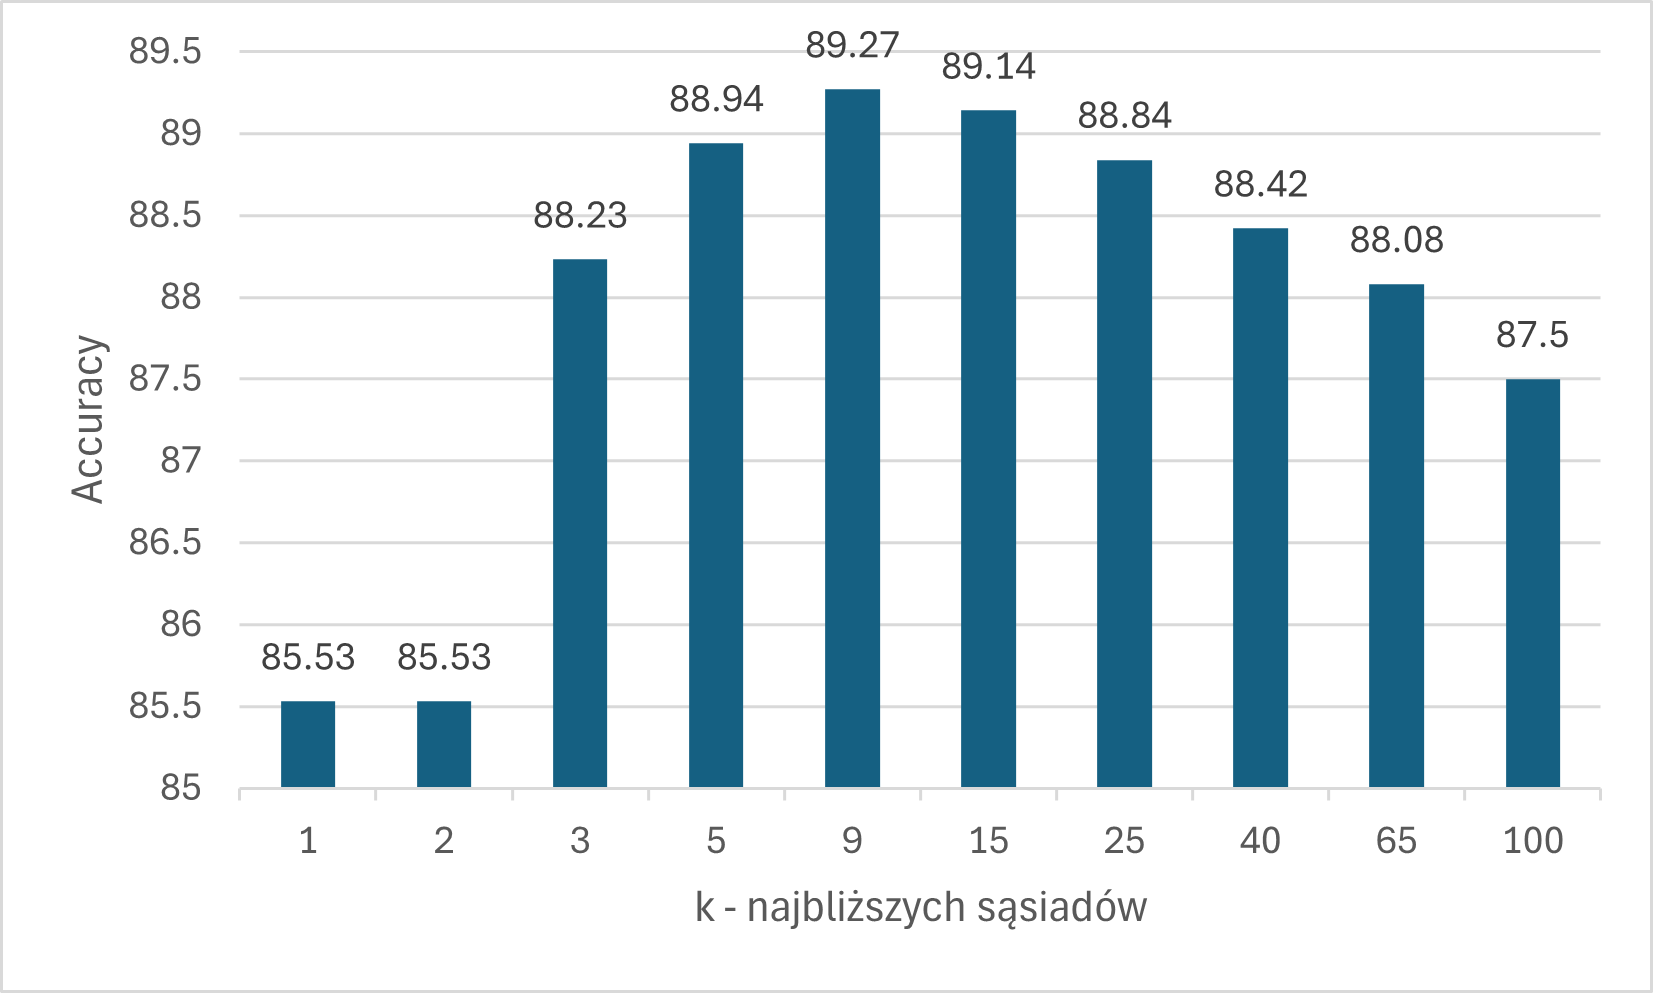
\includegraphics[width=\textwidth]{ksr/img/ACC - K.png}
%     \caption{Zależność accuracy do parametru k}
%     \label{fig:moj-obraz}
% \end{figure}

\subsection{Różny podział zbioru pomiędzy uczący, a testowy}
W poniższej tabeli przedstawiono wpływ proporcji podziału zbioru na dokładność klasyfikacji tekstów. Eksperymenty przeprowadzono przy stałych pozostałych ustawieniach: \(k\) = 9, metryce euklidesowej oraz zakresie długości n-gramów od \(n_1 = 2\) do \(n_2 = 4\).

\begin{table}[H]
    \centering
    \begin{tabular}{|c|c|c|c|c|c|c}
    \hline
    \textbf{Zbiór uczący[\%]} & \textbf{\(10\)} & \textbf{\(30\)} & \textbf{\(50\)} & \textbf{\(70\)}  & \textbf{\(90\)} \\ \hline
    \textbf{Zbiór testowy[\%]} & \textbf{\(90\)} & \textbf{\(70\)} & \textbf{\(50\)} & \textbf{\(30\)}  & \textbf{\(10\)} \\ \hline
    ACC [\%] & 87,91 & 88,74 & 89,17 & 89,27 & 88,80\\ \hline
    PPV\(_U\) & 0,8887 & 0,9009 & 0,9051 & 0,9072 & 0,9042\\ \hline
    TPR\(_U\) & 0,9803 & 0,9781 & 0,9785 & 0,9788 & 0,9804\\ \hline
    F1\(_U\) & 0,9323 & 0,9379 & 0,9404 & 0,9416 & 0,9408\\ \hline
    PPV\(_C\) & 0,8310 & 0,7650 & 0,7500 & 0,7770 & 0,7255\\ \hline
    TPR\(_C\) & 0,4104 & 0,4692 & 0,4877 & 0,4713 & 0,4512\\ \hline
    F1\(_C\) & 0,5495 & 0,5817 & 0,5910 & 0,5867 & 0,5564\\ \hline
    PPV\(_{UK}\) & 0,8046 & 0,8111 & 0,8590& 0,8390 & 0,8197\\ \hline
    TPR\(_{UK}\) & 0,5153 & 0,5757 & 0,5916 & 0,6324 & 0,5495\\ \hline
    F1\(_{UK}\) & 0,6283 & 0,6734 & 0,7007 & 0,7212 & 0,6579\\ \hline
    PPV\(_F\) & 0,7589 & 0,7807 & 0,8025 & 0,7358 & 0,8000\\ \hline
    TPR\(_F\) & 0,3761 & 0,5057 & 0,5159 & 0,5132 & 0,4615\\ \hline
    F1\(_F\) & 0,5030 & 0,6138 & 0,6280 & 0,6047 & 0,5854\\ \hline
    PPV\(_W\) & 0,7857 & 0,8333 & 0,8065 & 0,8421 & 0,7000\\ \hline
    TPR\(_W\) & 0,0379 & 0,1549 & 0,1553 & 0,1649 & 0,2121\\ \hline
    F1\(_W\) & 0,0724 & 0,2612 & 0,2604 & 0,2759 & 0,3256\\ \hline
    PPV\(_J\) & 0,8145 & 0,8333 & 0,8140 & 0,8140 & 0,8269\\ \hline
    TPR\(_J\) & 0,8571 & 0,8563 & 0,9013 & 0,9013 & 0,9149\\ \hline
    F1\(_J\) & 0,8353 & 0,8446 & 0,8554 & 0,8554 & 0,8687\\ \hline
    PPV\(_a\) & 0,8139 & 0,8207 & 0,8228 & 0,8182 & 0,7961 \\ \hline
    TPR\(_a\) & 0,5301 & 0,5900 & 0,6050 & 0,6053 & 0,5949\\ \hline
    F1\(_a\) & 0,5870 & 0,6521 & 0,6627 & 0,6614 & 0,6558\\ \hline
    \end{tabular}
    \caption{Wyniki miar przy badaniu wpływu podziału zbiorów na jakość klasyfikacji}
\end{table}

Wykres prezentujący zależność \(accuracy\) od podziału zbioru jest dostępny w załączniku o nazwie accuracy\_podzial.png.


\subsection{Różne metryki}
W poniższej tabeli przedstawiono wpływ różnych metryk na dokładność klasyfikacji tekstów. Eksperymenty przeprowadzono przy stałych pozostałych ustawieniach: podziale zbioru danych na 60\% zbioru uczącego i 40\% zbioru testowego \(k = 9\) oraz zakresie długości n-gramów od \(n_1 = 2\) do \(n_2 = 4\). \\

\begin{table}[H]
    \centering
    \begin{tabular}{|c|c|c|c|}
    \hline
    \textbf{Metryka} & \textbf{Euklidesowa} & \textbf{Uliczna} & \textbf{Czebyszewa}  \\ \hline
    ACC [\%] & 89,27 & 88,12 & 79,96\\ \hline
    PPV\(_U\) & 0,9061 & 0,8893 & 0,7988\\ \hline
    TPR\(_U\) & 0,9796& 0,9850 & 0,9998\\ \hline
    F1\(_U\)  & 0,9414& 0,9347 & 0,8881\\ \hline
    PPV\(_C\) & 0,7585& 0,7986 & 1,0000\\ \hline
    TPR\(_C\) &  0,4831& 0,3538 & 0,0092\\ \hline
    F1\(_C\) & 0,5902& 0,4904 & 0,0183\\ \hline
    PPV\(_{UK}\) & 0,8465& 0,8221 & 1,0000\\ \hline
    TPR\(_{UK}\) & 0,5939& 0,5746 & 0,0221\\ \hline
    F1\(_{UK}\) & 0,6981& 0,6764 & 0,0432\\ \hline
    PPV\(_F\) & 0,8000& 0,8679 & 0,0000\\ \hline
    TPR\(_F\) & 0,5545& 0,4554 & 0,0000\\ \hline
    F1\(_F\) & 0,6550& 0,5974 & 0,0000\\ \hline
    PPV\(_W\) & 0,8750& 0,7143 & 0,0000\\ \hline
    TPR\(_W\) & 0,1628& 0,0388 & 0,0000\\ \hline
    F1\(_W\) & 0,2745& 0,0735 & 0,0000\\ \hline
    PPV\(_J\) & 0,8168& 0,8289 & 0,8889\\ \hline
    TPR\(_J\) & 0,8824& 0,8289 & 0,0856\\ \hline
    F1\(_J\) & 0,8483 & 0,8289 & 0,1561\\ \hline
    PPV\(_a\) & 0,8338 & 0,8202 & 0,6146\\ \hline
    TPR\(_a\) &  0,6094 & 0,5394 & 0,1861\\ \hline
    F1\(_a\) & 0,6679 & 0,6002 & 0,1843\\ \hline
    \end{tabular}
    \caption{Wyniki miar przy badaniu wpływu metryk na jakość klasyfikacji}
\end{table}\

Wykres prezentujący zależność \(accuracy\) od metryki jest dostępny w załączniku o nazwie accuracy\_metryka.png.

% \begin{figure}[H]
%     \centering
%     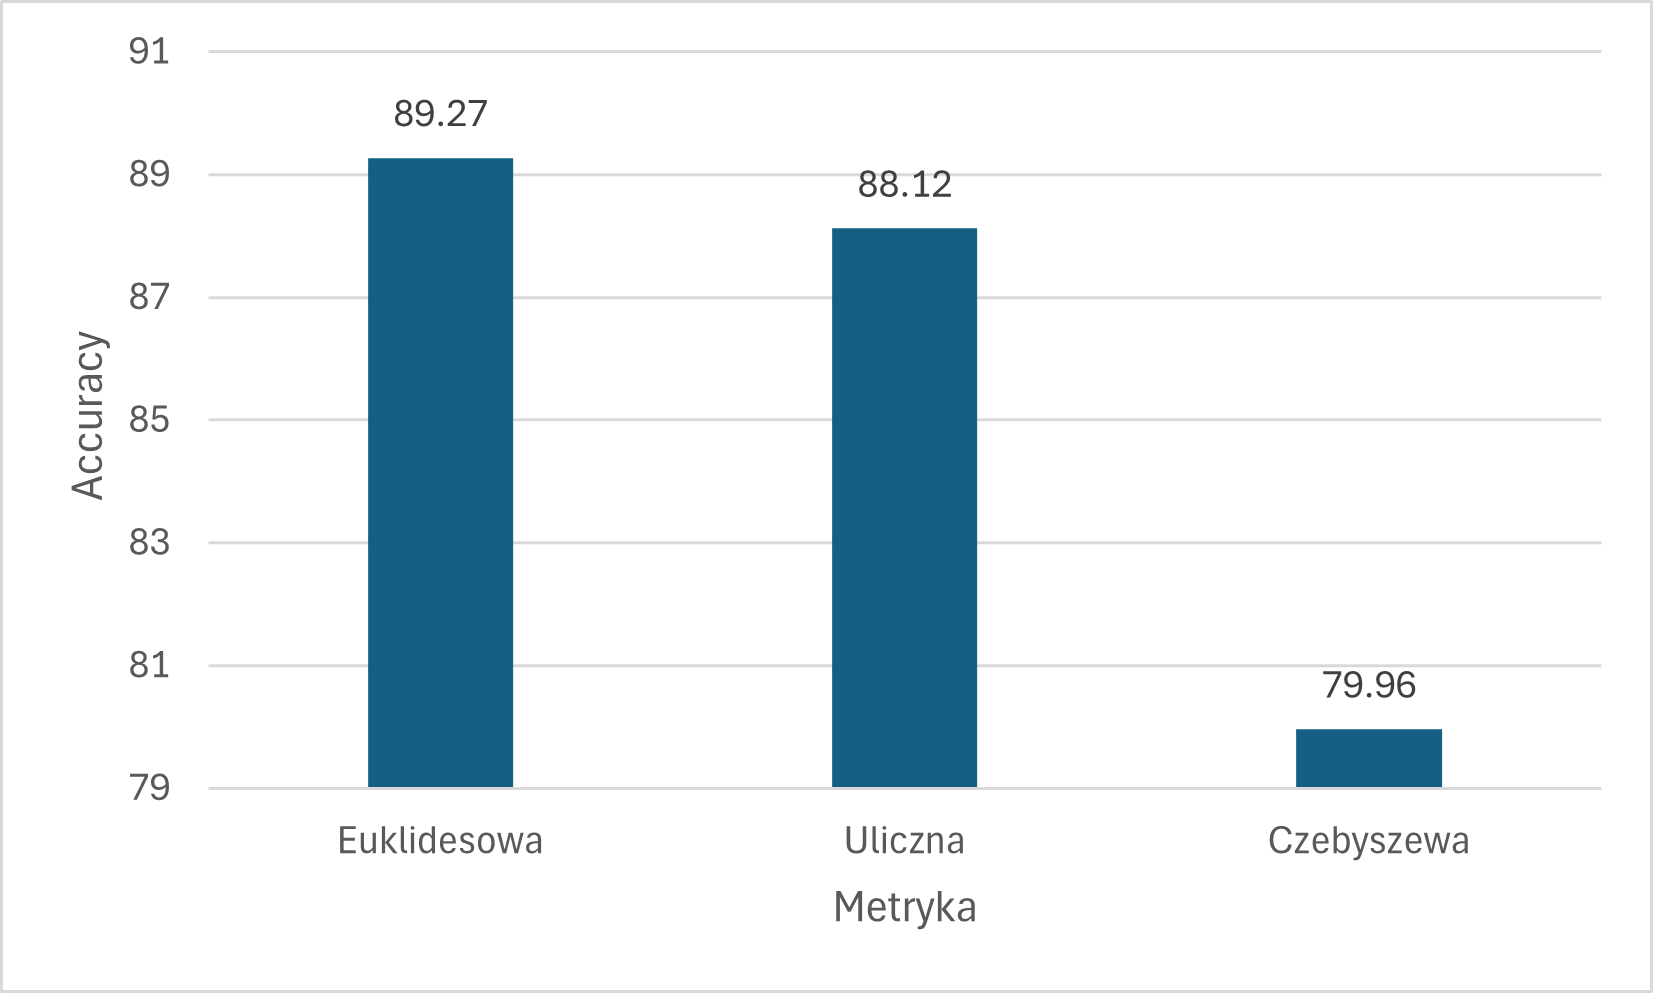
\includegraphics[width=\textwidth]{ksr/img/ACC - metryka.png}
%     \caption{Zależność accuracy do wybranej metryki}
%     \label{fig:moj-obraz}
% \end{figure}

\subsection{Dobór cech}
W poniższej tabeli przestawiono wpływ usunięcia różnych cech z wektora podstawowego na dokładność klasyfikacji tekstów. Eksperymenty przeprowadzono przy stałych pozostałych ustawieniach: podziale zbioru danych na 60\% zbioru uczącego i 40\% zbioru testowego \(k = 9\), metryce euklidesowej oraz zakresie długości n-gramów od \(n_1 = 2\) do \(n_2 = 4\). \\
Wykorzystane zostały cztery podzbiory cech, w których z głównego wektora usunięto:
\begin{enumerate}
    \item Dwie cechy tekstowe i dwie liczbowe - nazwiska, pierwsze słowo kluczowe w tekście, średnia długość słowa, liczba unikalnych słów
    \[
    v_1 = [ 0.04584717607973422, dlrs, [ florida, florida], 0.5597984105446793, 
    \]
    \[
         0.047619047619047616, 0.036312849162011177, 0.15584415584415584 ]
    \]
    \item Wszystkie cechy tekstowe - dominująca waluta, pierwsze słowo kluczowe w tekście, nazwy miejsca, nazwiska
    \[
    v_2 = [ 0.04584717607973422, 0.09576427255985268, 0.5597984105446793, 
    \]
    \[
          0.047619047619047616, 0.036312849162011177, 0.058823529411764705, 
    \]
    \[
        0.15584415584415584 ]
    \]
    \item Wszystkie cechy liczbowe - długość tekstu, liczba unikalnych słów, średnia długość słowa, liczba słów kluczowych w pierwszych 3 zdaniach, liczba słów zaczynających się wielką literą, liczba słów kluczowych, względna liczba słów kluczowych
    \[
    v_3 = [  dlrs, [ florida, florida], 0.09576427255985268, florida, [] ]
\]
    \item Dwie cechy tekstowe i dwie liczbowe - dominująca waluta, nazwy miejsca, średnia długość słowa, liczba unikalnych słów
    \[
    v_4 = [ 0.04584717607973422, 0.09576427255985268, 0.5597984105446793, 
\]
\[
     0.047619047619047616, 0.036312849162011177, florida, [] ]
\]
\end{enumerate}
\begin{table}[H]
    \centering
    \begin{tabular}{|c|c|c|c|c|c|}
    \hline
    \textbf{Podzbiór cech} & \textbf{\(v\)} & \textbf{\(v1\)} & \textbf{\(v2\)} & \textbf{\(v3\)} & \textbf{\(v4\)}  \\ \hline
    ACC [\%] & 89,27 & 88,42 & 79,21 & 88,45 & 87,76\\ \hline
    PPV\(_U\) & 0,9061 &0,9003& 0,8896 & 0,8927 & 0,8880 \\ \hline
    TPR\(_U\) & 0,9796 &0,9764 & 0,9672 & 0,9834 & 0,9846\\ \hline
    F1\(_U\)  & 0,9414 &0,9368 & 0,9268 & 0,9359 & 0,9338\\ \hline
    PPV\(_C\) & 0,7585 &0,7437 & 0,2162 & 0,7650 & 0,8163\\ \hline
    TPR\(_C\) & 0,4831 &0,4554 & 0,0246 & 0,4708 & 0,3692\\ \hline
    F1\(_C\) & 0,5902 &0,5649 & 0,0442 & 0,5829 & 0,5085\\ \hline
    PPV\(_{UK}\) & 0,8465 &0,8421 & 0,2817 & 0,9021 & 0,8128\\ \hline
    TPR\(_{UK}\) & 0,5939 &0,5746 & 0,0552 & 0,4834 & 0,4917\\ \hline
    F1\(_{UK}\) & 0,6981 &0,6831 & 0,0924 & 0,6295 & 0,6127\\ \hline
    PPV\(_F\) & 0,8000 &0,8800 & 0,5000 & 0,8154 & 0,7000\\ \hline
    TPR\(_F\) & 0,5545 &0,4356 & 0,0099 & 0,5248 & 0,4851\\ \hline
    F1\(_F\) & 0,6550 &0,5828 & 0,0194 & 0,6386 & 0,5731\\ \hline
    PPV\(_W\) & 0,8750 &0,6136 & 0,5588 & 0,9524 & 0,6452\\ \hline
    TPR\(_W\) & 0,1628 &0,2093 & 0,1473 & 0,1550 & 0,1550\\ \hline
    F1\(_W\) & 0,2745 &0,3121 & 0,2331 & 0,2667 & 0,2500\\ \hline
    PPV\(_J\) &  0,8168 &0,7635 & 0,3030 & 0,8053 & 0,8430\\ \hline
    TPR\(_J\) & 0,8824 &0,8289 & 0,0535 & 0,8182 & 0,7754\\ \hline
    F1\(_J\) & 0,8483 & 0,7949 & 0,0909 & 0,8117 & 0,8078\\ \hline
    PPV\(_a\) & 0,8338 & 0,7906 & 0,4446 & 0,8555 & 0,7842 \\ \hline
    TPR\(_a\) &  0,6094 & 0,5800 & 0,2123 & 0,5726 & 0,5435\\ \hline
    F1\(_a\) & 0,6679 & 0,6458 & 0,2278 & 0,6442 & 0,6143\\ \hline
    \end{tabular}
    \caption{Wyniki miar przy badaniu wpływu doboru cech na jakość klasyfikacji}
\end{table}

% \begin{figure}[H]
%     \centering
%     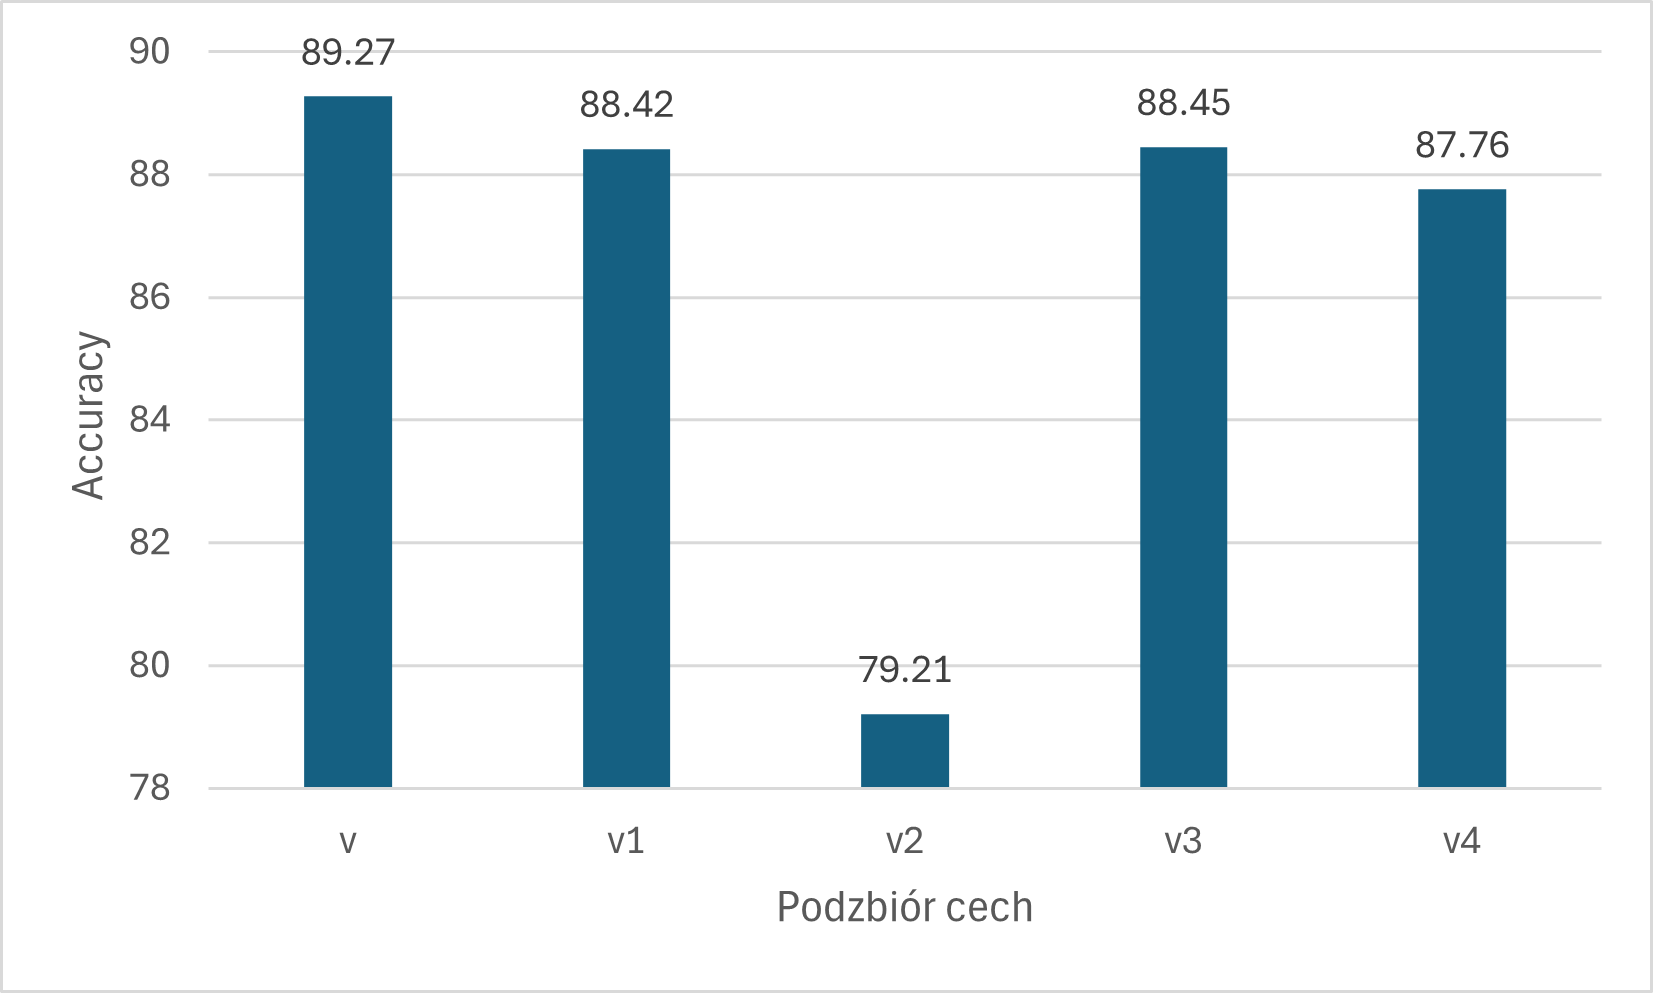
\includegraphics[width=\textwidth]{ksr/img/ACC - cechy.png}
%     \caption{Zależność accuracy do wybranej podzbioru cech}
%     \label{fig:moj-obraz}
% \end{figure}

Wykres prezentujący zależność \(accuracy\) od podziału zbioru jest dostępny w załączniku o nazwie accuracy\_cechy.png.

\section{Dyskusja, wnioski, sprawozdanie końcowe}
\subsection{Wpływ parametru k na jakość klasyfikacji}
Na podstawie rysunku dostępnego w załączniku pod nazwą accuracy\_k.png można zaobserwować, że miara \(accuracy\) rośnie wraz ze wzrostem parametru \(k\) do wartości \(k = 9\), osiągając wówczas wartość maksymalną. Dalsze zwiększanie parametru \(k\) prowadzi do stopniowego pogorszenia dokładności klasyfikatora. Aby jednak w pełni ocenić wpływ parametru \(k\) na jakość klasyfikacji, należy również przeanalizować miary \(recall\), \(precision\) oraz \(F1\), które są obliczane oddzielnie dla każdej klasy. \\
Analiza danych z tabel 2 i 3 wskazuje, że wartość \(precision\) dla klasy USA maleje wraz ze wzrostem \(k\), natomiast dla pozostałych klas zachowuje się nieregularnie. Wartości skrajne, takie jak 1 lub 0, pojawiają się w przypadkach, gdy liczba zaklasyfikowanych dokumentów do danej klasy jest bardzo mała. Na przykład, precyzja dla klasy Niemcy Zachodnie wynosi 1 przy \(k = 65\), a 0 przy \(k = 100\), co oznacza, że przy większym \(k\) żaden artykuł nie został zaklasyfikowany jako należący do tej klasy. Takie zachowanie wynika z przewagi liczebnej klasy USA, co skutkuje częstszym przypisywaniem dokumentów właśnie do niej. \\ 
Dla miary \(recall\) obserwuje się stopniowy wzrost dla klasy USA i Japonii, co oznacza coraz lepsze rozpoznawanie dokumentów należących do tych klas. Dla pozostałych klas czułość utrzymuje się na stabilnym poziomie przy małych wartościach \(k\), po czym maleje przy większych wartościach. W skrajnych przypadkach, jak dla klasy Niemiec Zachodnich, \(recall\) osiąga 0, co świadczy o całkowitym braku prawidłowych przypisań do tej klasy.\\
Zaobserwowane zjawiska wynikają głównie z dominacji klasy USA, która stanowi około 79\% wszystkich dokumentów w zbiorze. Sytuacja ta pokazuje, że wysoka wartość jednej z miar, np. \(recall\) czy \(precision\), nie zawsze świadczy o dobrej jakości klasyfikatora. W takich przypadkach szczególnie użyteczna jest miara \(F1\), która pozwala ocenić równowagę pomiędzy precyzją a czułością. Najwyższe wartości tej miary uzyskano przy \(k = 9\) dla czterech klas, natomiast dla klasy Niemiec Zachodnich i Japonii wartości maksymalne występują odpowiednio przy \(k = 5\) oraz \(k = 15\). \\
Na podstawie przeprowadzonych analiz można stwierdzić, że optymalna wartość parametru \(k\) powinna być ustalana nie tylko na podstawie miary \(accuracy\), ale również z uwzględnieniem metryk klasyfikacyjnych obliczanych osobno dla każdej klasy. W przypadku tego doświadzenia jest to k z zakresu 5 - 15.

\subsection{Wpływ podziału zbiorów na jakość klasyfikacji}
Na rysunku dostępnym w załączniku o nazwie accuracy\_podzial.png został zaprezentowany wpływ różnego podziału zbioru na uczący oraz testowy. Można zauważyć, że wraz ze wzrostem procentowego udziału zbioru treningowego, miara \(accuracy\) stopniowo rośnie do wartości 89{,}27\% przy podziale 70/30, po czym nieznacznie spada dla proporcji 90/10. Różnice te są jednak niewielkie – maksymalna różnica między najlepszym a najgorszym wynikiem wynosi ok. 1,3 p.p. \\
Dla klasy dominującej (USA) miary jakości klasyfikacji (\(precision\), \(recall\), \(F1\)) są bardzo wysokie i stabilne niezależnie od proporcji danych, co wynika z dużej liczebności tej klasy w zbiorze. \\
W przypadku pozostałych klas, które są mniej liczebne, sytuacja jest bardziej złożona. Miara \(precision\) zachowuje się niestabilnie – wartości rosną i maleją w zależności od podziału danych. Natomiast miara \(recall\) zazwyczaj wzrasta do momentu osiągnięcia proporcji 50/50 lub 70/30, po czym nieco spada. \\
Na podstawie powyższych obserwacji można stwierdzić, że optymalny kompromis pomiędzy liczbą przykładów uczących a jakością klasyfikacji występuje przy podziale 70/30 lub 50/50. Natomiast zbyt mała liczebność zbioru uczącego jest najbardziej niekorzystna dla klas z najmiejszą liczbą obiektów, w przypadku tego doświadczenia jest to Francja oraz Niemcy Zachodnie.

\subsection{Wpływ wyboru metryki na jakość klasyfikacji}
Na rysunku dostępnym w załączniku o nazwie accuracy\_metryka.png przedstawiono porównanie wartości \(accuracy\) przy użyciu różnych metryk odległości. Można zauważyć, że dla metryki euklidesowej uzyskano najlepszy wynik, nieco niższy (o ok. 1 p.p.) dla metryki ulicznej oraz znacznie niższy (o ok. 10 p.p.) dla metryki Czebyszewa.\\
W przypadku klasy dominującej (USA), zgodnie z tabelą 5, zmiana metryk z euklidesowej na uliczną, a następnie na Czebyszewa prowadzi do pogorszenia miary \(precision\), ale jednocześnie do poprawy miary \(recall\), jednak miara \(F1\) wskazuje jednoznacznie, że najlepszą równowagę pomiędzy precyzją a czułością osiągnięto dla metryki Euklidesowej. \\
Metryka uliczna, choć osiąga niższe wyniki dokładności niż euklidesowa, wykazuje w niektórych przypadkach lepszą precycję kosztem nieco niższej czułości. Niemniej jednak ogólny poziom \(F1\) pozostaje niższy niż dla metryki euklidesowej. \\
Z kolei metryka Czebyszewa dla klas mniej licznych niż USA prowadzi do skrajnych wyników. Przykładowo, dla Kanady precyzja osiąga wartość 1, podczas gdy dla Francji wynosi 0. Jednocześnie w przypadku czułości wartości są bardzo niskie lub bliskie zeru. Jest to związane z dużą czułością metryki Czebyszewa na brak podobieństwa pojedynczych cech składowych wektorów cech. Dla przykładu, dziewięć cech może wskazywać na duże podobieństwo pomiędzy artykułami, jednak jedna cecha o zerowym podobieństwie znacząco obniża wynik całkowity. W konsekwencji większość tekstów jest klasyfikowana jako USA, czyli do klasy dominującej liczebnie.

\subsection{Wpływ doboru cech na jakość klasyfikacji}
Na rysunku dostępnym w załączniku pod nazwą accuracy\_cechy.png przedstawiono wykres wartości \(accuracy\) przy użyciu różnych podzbiorów cech. Można zauważyć, że w przypadku usunięcia dwóch cech tekstowych i dwóch liczbowych oraz  wszystkich cech liczbowych spadek dokładności klasyfikatora nie jest znaczący - w najgorszym przypadku wynosi ok. 1.7 p.p. Wyraźne pogorszenie dokładności obserwuje się natomiast po usunięciu wszystkich cech tekstowych. \\
Zgodnie z tabelą 6, dla wektora cech \(v1\) miary \(precision\), \(recall\) oraz \(F1\) dla większości krajów spadają. Natomiast dla wektora \(v4\) zmiany tych miar są bardziej nieregularne, w niektórych przypadkach obserwuje się wyraźne spadki, a w innych — poprawę, np. precyzji dla Kanady. Na tej postawie można dojść do wniosku, że cechy tekstowe, których brak obserwujemy w wektorze \(v4\) mają istotniejszy wpływ na jakość klasyfikacji. \\
Usunięcie wszystkich cech liczbowych \(v3\) wpływa w niewielkim stopniu na wartości miar jakości klasyfikacji dla większości krajów. Wyjątkiem jest Wielka Brytania, dla której precyzja znacząco wzrasta przy jednoczesnym spadku czułości, co ostatecznie obniża wartość miary \(F1\). \\
W przypadku usunięcia wszystkich cech tekstowych \(v2\) wartości miar jakości klasyfikacji dla wszystkich krajów, poza USA, drastycznie spadają. Na podstawie powyższych obserwacji można stwierdzić, że cechy tekstowe mają kluczowy wpływ na skuteczność klasyfikacji metodą KNN.

\subsection{Wnioski}
\begin{itemize}
    \item Niezrównoważone dane (dominacja jednej klasy) powodują, że klasyfikator KNN jest skłonny przypisywać większość obiektów do liczniejszej klasy, co znacząco obniża wartości miar jakości klasyfikacji metodą KNN.
    \item Wartość parametru k ma znaczący wpływ na jakość klasyfikacji metodą KNN, dlatego należy starannie go określić.
    \item Wnioski o jakości klasyfikacji nie powinny być oparte wyłącznie na wartości \(accuracy\), ponieważ w przypadku nierównomiernego rozkładu klas może ona być myląca. Warto analizować również \(precison\), \(recall\) i \(F1\).
    \item Wybór metryki odległości wpływa na wyniki klasyfikacji — metryki takie jak uliczna lub Euklidesowa dają bardziej stabilne wyniki w porównaniu do metryki Czebyszewa, która jest bardziej podatna na duże różnice w pojedynczych cechach.
    \item Cechy tekstowe dostarczają istotniejszych informacji o klasyfikowanych obiektach niż cechy liczbowe, co jest widoczne poprzez większe pogorszenie jakości klasyfikacji po ich usunięciu.
    \item Etap doboru cech powinnien być przeprowadzana ostrożnie, ponieważ prawidłowy dobór cech jest konieczny do uzyskania wysokiej jakości klasyfikacji metodą KNN.
\end{itemize}


\begin{thebibliography}{0}
\bibitem{reuters} Reuters-21578 Text Categorization Collection,\url{https://archive.ics.uci.edu/dataset/137/reuters+21578+text+categorization+collection} [dostęp 27.04.2025r.]
\bibitem{knn} Metoda k-NN \url{https://home.agh.edu.pl/~horzyk/lectures/miw/KNN.pdf} [dostęp: 28.03.2025r.]
\bibitem{tab} Wikipedia, Tablica pomyłek, \url{https://pl.wikipedia.org/wiki/Tablica_pomy%C5%82ek}. [dostęp: 28.03.2025r.]
\bibitem{wyklad} A.Niewiadomski, Materiały wykładowe do przedmiotu Komputerowe Systemy Rozpoznawaniam, ksr-wyklad-2009 \url{https://ftims.edu.p.lodz.pl/mod/folder/view.php?id=135292} [dostęp 27.04.2025r.]
\end{thebibliography}

\end{document}